\documentclass{report}

\usepackage{import}
\import{../}{gov-style}
\addbibresource{../thesis.bib}

\begin{document}
\section{Introduction}
\subsection{In space, no one will shoot you down}
Six flags rest on the surface of the moon: one fallen, five standing, and all American.\footnote{Well, they \emph{were} American. All of the flags are now bleached white after years of direct exposure to sunlight. (\cite{spudis_faded_2011})} Like the antarctic and the open seas, every nation may explore the moon, but none have the right to own it. Were China to launch a manned lunar mission tomorrow, and plant their own flag on the surface of the moon, no one would question their right to do so, but no one would interpret that as a claim to ownership either. The history of human activity in space follows that exact pattern. A state has the essentially unquestioned right to put anything in space, so long as it does not interfere with something that another state has already placed there. The Outer Space Treaty (OST), which entered into force only ten years after \emph{Sputnik}, formalized this practice: ``Outer space \textelp{} is not subject to national appropriation by claim of sovereignty, by means of use or occupation, or by any other means.''\footcite{noauthor_outer_1966} The strength of the OST has never been tested. Not once in the history of human space activity have hostile forces disabled, damaged, or destroyed an object in space that was not their own.

While it makes perfect sense that no state has attempted to enforce a territorial claim on the moon---technological feasibility aside, there's not much up there worth fighting for---artificial satellites present a much more tempting target. Satellites are numerous, accessible, and undergird essential civil infrastructure. If a nation were so inclined, removing key satellites controlled by their adversaries could give them a significant strategic advantage. That an equilibrium held throughout the Cold War in which all satellites---regardless of their applicability to military, commercial, or scientific ends---were left undisturbed is one of the most remarkable achievements of the international system. The world today relies on communication infrastructure that only exists because the safety of the satellites that make them possible is functionally guaranteed by decades of peace in outer space.

At the dawn of the space age, the safety of artificial satellites was far from guaranteed. Four years after the first U-2 mission, a familiar dynamic could have played out when the first spy satellite launched in August 1960: the US develops a new photo-reconnaissance technology which its main adversary is unable to prevent; the USSR diplomatically objects to the technology's use; the USSR finally develops a weapon capable of counteracting the new technology; and the USSR employs it. Each one of these steps came to pass except the last---even after developing a feasible ASAT weapon, the Soviet Union never made use of it. And the onus was on them to push back against the American efforts to normalize satellite reconnaissance. \emph{Sputnik} briefly put the USSR at the forefront of the final frontier, but the satellite itself was totally innocuous; it obtained data about the density of the atmosphere and propagation of radio waves.\footcite{nasa_sputnik_2019} It was the United States that would first launch a satellite capable of photo-reconnaissance---and it was the Soviet Union that would let them get away with it.

Spy satellites are not just one of the best edge cases for norm against shooting down a satellite, they are the reason it exists in the first place.\footnote{I'm not suggesting that, absent spy satellites, nations would have just constantly shot down each other's weather satellites. But remember that the CIA planned a cover for the U-2 in which it was a ``weather plane'' that had gone off course. The USSR forced a cargo plane to land in Hungary because they suspected it of espionage. That never happens in space, because intelligence norms are strong enough that the accusation of dual-use is never even raised. There are no good and bad satellites; as long as a satellite doesn't have literal weapons, then there is no plausible reason to shoot it down.} The reconnaissance satellite succeeded because the Eisenhower administration purposefully designed its space program to establish a norm of peaceful development---with the single goal of legitimizing satellites for intelligence-gathering. While these intelligence norms limit the diplomatic response to other forms of espionage, such as reconnaissance flights and human espionage, they cannot eliminate the response entirely, because those activities run afoul of longstanding principles regarding territorial integrity and domestic law. In space, where no such principles existed previously, the only established norm at the dawn of the space age was one from the world of espionage---that intelligence-gathering entities are not inherently aggressive. Thus space became an environment where a strike against a satellite would constitute the first act of aggression, even though the satellite was potentially gathering information that could significantly compromise a state's security position. In their success, the United States finally gained unrestricted access to aerial intelligence of the type that an Open Skies policy might have provided. That all satellites, regardless of purpose, are immune to hostilities as a result is just a happy byproduct.

In this chapter I will interrogate how the norm against using anti-satellite (ASAT) weapons managed to hold throughout the entire Cold War, and how it continues to do so today. Unlike in previous chapters, it is not necessary to prove that there is a muted diplomatic response to satellite espionage because the lack of response is self-evident: no military action has ever been taken against satellites, and the Soviet Union only objected to reconnaissance satellites until they were able to make their own. The first section will demonstrate how Eisenhower designed the rollout of the American satellite program with an eye towards influencing international law, developing a norm that would permit reconnaissance satellites. The section after will examine how the norm preserving intelligence capabilities was a significant factor in preventing the weaponization of space during the 1980s. And the final section discusses how well that norm is performing today.

\section{Framing the spy satellite}
\subsection{Planning for a new security environment}
The successful launch of a spy satellite, in 1960, was nothing less than the culmination of a decade-long grand strategy to secure The United States of America against a surprise nuclear attack. Though the US air-atomic capabilities in the early Cold War discouraged the USSR from making more use of their conventional military advantage, the USSR quickly developed their own nuclear weapons and was rapidly developing longer-ranged delivery systems. The fear of a surprise nuclear attack haunted Eisenhower throughout his presidency.\footcite[p.~68]{killian_sputnik_1977} American status and security relied on the ability to accurately asses Soviet capabilities and foresee such an attack, and producing those accurate assessments required state-of-the-art intelligence.

As detailed in previous chapters, the closed nature of the Soviet state posed a significant challenge to American intelligence efforts. One of the highest priority goals of the Eisenhower administration's foreign policy was to permanently rectify this imbalance by opening up the Soviet state to photo-reconnaissance.\footcite[p.~65]{hayes_struggling_1994} With little information emerging from the USSR of its own volition, and the difficulty of running human agents deep within a paranoid surveillance state, some novel technical approaches would be required. Spy planes, artificial satellites, and other then-futuristic reconnaissance possibilities had been discussed since the end of WWII, but they remained theoretical concepts for many years. That all changed in 1954, when Eisenhower met with the Office of Defense Mobilization's Science Advisory Committee, and requested that they put together a task force which would tackle the problem of America's vulnerability to a surprise attack.\footcite[p.~67. The president's science advisor described this moment as the starting point for ``any complete account of how science advice was mobilized for the use of President Eisenhower.'']{killian_sputnik_1977}

Chaired by MIT President Dr. James Killian, the Technological Capabilities Panel (TCP) was tasked with forecasting America's strategic position and presenting possible technical solutions to mitigate the threat of a nuclear Pearl Harbor.\footcite[p.~115]{mcdougall_heavens_1985} They presented their results in February 1955---a report formally titled ``Meeting the Threat of a Surprise Attack,'' but also variously referred to as the ``Killian Report,'' ``TCP Report,'' or ``Surprise Attack Study.'' The report predicted four distinct periods of relative power would unfold over the next decade, starting with the current era in which neither side of the Cold War was capable of a decisive strike but the US had a relative advantage in air-atomic power, and ending in a world where mutual ICBM capabilities ensured that the balance of power would remain a stalemate indefinitely.\footcite[p.~116]{mcdougall_heavens_1985}

All four Cold War phases that the Killian Report predicted---with shocking accuracy, as it turned out---had one thing in common: the sobering calculation that a great power conflict would result in heavy American losses. Even in the phase where American relative power was to be at its greatest (before the development of Soviet multimegaton capability), the United States ``would be severely damaged,'' and ``emerge a battered victor'' in the event of a surprise attack.\footcite{technological_capabilities_panel_meeting_1955} Killian wrote that, while presenting the report to the National Security Council (NSC), ``we emphasized that even though our \emph{relative} military strength might change in the manner suggested in the table, we still would be in a position where the United States could be grievously hurt.''\footcite[p.~75]{killian_sputnik_1977}

Therefore it was of paramount importance to avoid a general conflict at all costs, and the report was split into different subgroups that approached the problem from all angles. One subgroup, for instance, analyzed the progress of American ICBMs, in order to match Soviet capabilities and discourage a first-strike. But not all of them were focused on offensive capabilities. Another subgroup devoted themselves to studying novel approaches for intelligence-gathering. ``We \emph{must} find ways to increase the number of hard facts upon which our intelligence estimates are based,'' the Intelligence Section states, ``to provide better strategic warning, to minimize surprise in the kind of attack, and to reduce the danger of gross overestimation or gross underestimation of the threat.''\footcite{technological_capabilities_panel_meeting_1955} The entire security position of the United States relied on the country developing scientific means to minimize the risk of miscalculation.

\subsection{The spy plane walked so the spy satellite could run}
One of the proposals to come out of the TCP recommendations is a project about which you have already read. The panel learned that the Air Force had rejected a proposal from Lockheed for a long-range, jet-powered glider. The scientists in charge of the Intelligence Section---led by Edwin Land, co-founder of Polaroid---realized that when equipped with photographic equipment and other intelligence devices, the Lockheed prototype had the potential to serve as a revolutionary information-gathering machine.\footcite[p.~81-82]{killian_sputnik_1977} They proposed that Eisenhower approve what came to be known as Project AQUATONE; the president accepted; and development of the U-2 spy plane began. At the same time, the Eisenhower's positive reaction to the Killian Report caused both the CIA and the Air Force to accelerate their existence plans for reconnaissance satellites.\footcite[p.~83]{killian_sputnik_1977}

The U-2 revolutionized aerial reconnaissance, but even in the early days when it remained literally untouchable, the intelligence that it provided had limitations. While the U-2 provided CIA imagery analysts with impossibly high-resolution photos of an individual military base, it was less helpful in determining the locations of various military bases throughout the vast expanse of Soviet territory, a task for which satellites showed enormous potential. The spy plane offered depth; the spy satellite promised breadth. Together, they could operate for complementary purposes: a spy plane dispatched when high quality localized intelligence was required, and a satellite to form a more comprehensive picture of the Soviet military posture.

Even more important than the the technical benefits of a spy satellite were the potential political ones. Because the territorial boundary conditions of outer space were completely undefined, the spy satellite might able to perform photo-reconnaissance overflights with a consistency that a spy plane never could. When the U-2 started flying missions in 1956, it flew high enough to avoid Soviet anti-aircraft capabilities, but that status quo had a clear expiration date. The overflight program was so risky that it was originally intended to last only a year or two.\footcite[p.~33]{lindgren_trust_2000} The Soviets considered overflights to be a violation of their territorial sovereignty, and continued to register diplomatic protests about them. Satellites, by contrast, operated in a new space that had the potential to transcend airspace norms, where they could fly ``over'' Soviet territory with impunity. Here is historian Walter McDougall, writing about the promise of satellites in his book on the political history of the space age:

\begin{quote}
	If continuous surveillance of Soviet installations and exact targeting of Soviet bases were to be assured, the solution was to spy from outer space. Camera-toting satellites, circling the earth south to north [sic] in a polar orbit, could view the entire surface of the earth as it rotated below, return to any location in a few days' time, hone in on suspicious areas, and do it all under the legal cover of freedom of space---if such legal cover could be established. Given the simultaneous USAF go-ahead for Project WS-117L and Land's insistence on applying the most advanced knowledge of science and technology to intelligence, there is little doubt that the portions of the Killian Report that remain classified to this day include the recommendation that the highest national priority attach to the development and operation of reconnaissance satellites.\footcite[p.~117]{mcdougall_heavens_1985}
\end{quote}

The key phrase here is ``if such a legal cover could be established.'' The undefined legal status of space presented an opportunity, but also a challenge. The TCP understood that the Soviet Union would likely recognize the enormous advantage that such a satellite would confer on the US, and object to their deployment using any international norms possible.  It was therefore necessary to present reconnaissance satellites in such a way that would limit the grounds for objection. Fortunately, plans for that were already underway, and the TCP found them.

Though the Killian Report that first elevated the issue to a top national security priority, American policymakers had been considering how to politically frame the space program for years. The Air Force commissioned a series of studies about the potential for artificial satellites from 1946 to 1947, and concluded that they were feasible, but not necessarily practical.\footcite[p.~5-6]{peebles_corona_1997} Progress was limited until 1950, when  the Air Force again commissioned the RAND corporation to study the potential military utility of artificial satellites. The resulting report, according to McDougall, ``deserves to be considered the birth certificate of American space policy.''\footcite[p.~108]{mcdougall_heavens_1985} By my accounting, ``The Satellite Rocket Vehicle: Political and Psychological Problems'' should also be considered the birth certificate of American strategic intelligence policy---and the international norms that resulted.

The RAND report succinctly presented the challenges that intelligence norms faced at the outset of the Cold War, and the benefits that the US stood to gain by promoting them. The potential damage that spy satellites posed to the Soviet strategic posture was considerable, and the Soviet Union, politically and culturally, was singularly sensitive to invasions of privacy. ``Fear of loss of secrecy is constant and intense,'' it noted, and ``it is to be expected that attacks upon secrecy will be construed as attacks upon Soviet sovereignty.''\footcite[p.~14]{kecskemetic_satellite_1950} The RAND report predicted that the USSR will likely see a novel reconnaissance satellite as a major threat, altering the balance of power between the two states, and take the appropriate measures to counteract it.\footcite[p.~13]{kecskemetic_satellite_1950}

The report also made clear that, even before developing ASAT capabilities, the USSR would have plenty of options to put pressure on the United States that fell short of total war. They might pursue litigation in the International Criminal Court, the outcome of which would be uncertain, especially if there were evidence that the satellite was gathering intelligence.\footcite[p.~16]{kecskemetic_satellite_1950} Or, if the satellite required receiving stations in foreign countries, the USSR could put pressure on the host countries to shut the stations down, threaten to destroy the stations, or simply attack the stations with military force.\footcite[p.~16-17. Importantly, these are all things that the Soviet Union could have done with the U-2 spy plane as well. The US was somewhat more circumspect with its overflights, but the options were there. As it turned out, the first spy satellite, CORONA, ejected a film capsule and required no such receiving stations.]{kecskemetic_satellite_1950}

These results sparked a renewed Air Force interest in reconnaissance satellites, and the service began putting together the hardware specifications for one in 1951. These specifications became Project WS-117L, ``a strategic satellite system,'' and the first American space program.\footcite[p.~110-111. The WS is short for ``Weapons System.'']{mcdougall_heavens_1985} So when the members of the TCP began to survey the possibilities for the future of American strategic reconnaissance, they found Project WS-117L---exactly the kind of technical innovation that they were looking for.\footcite[p.~197]{brugioni_eyes_2010} But the United States could not begin the space age with a spy satellite. Doing so would ensure that outer space became yet another arena for conflict, the way airspace had at the turn of the \nth{20} century. What happened instead reflects incredible forethought on the part of Eisenhower and his administration, who baked intelligence norms into the legal framework of outer space, then launched a spy satellite into the legal regime that they created.

\subsection{Building the civilian space program}
Everything about the administration's space policy was carefully crafted to set the stage for the eventual launch of a spy satellite. From the time that artificial satellites first appeared viable until he left office, Eisenhower used the civilian space program as a public means of diverting attention from the security-related programs he valued.\footcite[p.~119]{day_eye_2015} Acting on the recommendations of the TCP, the National Security Council (NSC) proposed a scientific satellite program in May 1995, which Eisenhower accepted. In this memo, NSC-5520, the NSC Planning Board argued that, when framed properly, a scientific satellite could be used as diplomatic tool to promote a norm establishing ``freedom of space.'' The proposal tracks closely with a similar one from the 1950 RAND report, which suggested that the US first launch an innocuous ``experimental satellite'' that did not cross over Russian territory, and gauge the diplomatic reaction.\footcite[p.~21]{kecskemetic_satellite_1950} The political framing of the satellite is discussed at the top of NSC-5520, in a section entitled \emph{General Considerations} (emphasis mine):

\begin{quote}
6. \textelp{} \textbf{Furthermore, a small scientific satellite will provide a test of the principle of “Freedom of Space”. The implications of this principle are being studied within the Executive Branch.} However, preliminary studies indicate that there is no obstacle under international law to the launching of such a satellite.

7. \textbf{It should be emphasized that a satellite would constitute no active military offensive threat to any country over which it might pass.} Although a large satellite might conceivably serve to launch a guided missile at a ground target, it will always be a poor choice for the purpose. A bomb could not be dropped from a satellite on a target below, because anything dropped from a satellite would simply continue alongside in the orbit. \footcite{nsc_planning_board_draft_1955}
\end{quote}

What NSC-5520 did not anticipate was the the US wouldn't have to establish that principle on their own. Getting beaten to orbit by \emph{Sputnik} put the United States at an advantage. The Soviets could hardly denounce the American satellite program as suspicious when they very publicly made the first move---and without asking permission to orbit over the United States.\footcite[p.~40]{peebles_corona_1997} The US didn't \emph{try} to lose first leg of the space race, per se, but policymakers were aware of this dynamic well in advance. Reviewing NSC-5520, Nelson Rockefeller wrote that since the Soviets had already announced plans to launch a satellite, the existence of their project could be used to good effect against the inevitable Soviet protests about the American satellite program.\footcite[p.~120]{mcdougall_heavens_1985} Already variously occupied by the need to finish the ICBM, monitor Soviet R\&D, and frame the satellite program as a civilian scientific endeavor, the administration assigned the winning the space race to the lowest possible priority. Though ideally the US would be able to set the precedent for ``freedom of space''themselves, the senior administration understood that if the USSR launched first, it would clear the legal path for them. Using military technology in an effort to be first would remove that possibility and jeopardize the other objectives at the same time.\footcite[p.~123-124]{mcdougall_heavens_1985} Eisenhower himself repeatedly dismissed concerns about the prestige of being the first nation to orbit an object in space, and from the standpoint of international law, he might have been right.\footcite[p.~134]{day_eye_2015}

In fact, the overriding American priority to legitimize reconnaissance satellites is probably the \emph{reason} that the Soviets started the Space Age instead. Just as Eisenhower limited the involvement of the Air Force in AQUATONE to paint the U-2 as a civilian project, technical decisions were made to make the scientific satellite seem as non-threatening as possible, and none more important than the vehicle that would launch it. The group tasked with implementing NSC-5520 had to choose between competing launch proposals from the Army, Navy, and Air Force. They made the somewhat surprising choice to go with the unproven Navy Research Laboratory (NRL) \emph{Vanguard} rocket, even though the Army Ballistic Missile Agency (ABMA) engineers, headed by famous rocketeer Wernher von Braun, had been developing their proposal for a year. Among the reasons the committee gave for their decision, two stand out. First, the NRL impressed the committee with their plans for scientific components and a radio tracking system.\footcite[p.~122]{mcdougall_heavens_1985} Second, the panel purposefully wanted to avoid using a ballistic missile.\footcite[p.~129. Though the NRL is run by the Navy, it functions like a civilian scientific operation. Everything that I have read about this decision seems to take it for granted that despite the Navy involement, the NRL proposal would be seen as a civilian project, which makes sense to me, especially when compared to using the same agency that was building nuclear delivery systems.]{day_eye_2015}

Launching the first satellite with a ballistic missile threatened to compromise two of the American foreign policy priorities. It might delay the development of the ICBM, which posed an existential threat to American military superiority, and it would jeopardize the civilian character of the satellite program, which the committee members were determined to preserve.\footcite[p.~122]{mcdougall_heavens_1985} The Von Braun engineers vigorously protested the decision, because they believed---correctly---that their proposal would succeed first. But being first in space was not the goal, establishing a legal precedent was. Von Braun's appeals were continually rejected, and always for the same reason: launching a satellite with no scientific purpose other than demonstrating superiority would compromise the moral position that the US desperately needed to establish.\footcite[p.~131]{day_eye_2015}

Publicly, \emph{Vanguard} was a disaster. The rocket experienced an embarassing setback on December 6, 1957, when it failed to launch a three-and-a-half pound satellite, just after the USSR had successfully launched \emph{Sputnik II}.\footcite[p.~119]{killian_sputnik_1977} The Soviets had put a dog in space before the Americans even managed to get a satellite up there.\footcite[Her name was Laika.]{george_sad_2018} When then United States finally succeeded in launching at satellite, it was not thanks to the \emph{Vanguard}, but rather the ABMA team that had been consistently rebuffed by the administration. Finally given the chance, Von Braun and his engineers quickly accomplished what they had always said they would: modify a Jupiter-C ballistic missile to send a satellite into orbit. The Army launched \emph{Explorer 1} on January 31, and it carried a pioneering array of miniaturized electronics, including two micrometeoroid detectors and a Geiger counter.\footcite[p.~168]{mcdougall_heavens_1985} \emph{Explorer 1} and \emph{Vanguard 1}, which launched about six weeks later, provided an impressive amount of scientific data in comparison to the Sputniks.\footcite[p.~168]{mcdougall_heavens_1985} More importantly, even though the US did end up launching a satellite using a ballistic missile, their visible defeat in the space race and clear scientific purpose had the intended effect of blunting Soviet efforts to characterize the American satellite program as a military development. It was time to launch a spy satellite.

\subsection{CORONA}

\section{Reagan, Star Wars, and the fervor of space weaponization}
That peace is all the more remarkable when you consider that even though space has never been weaponized, it has been thoroughly \emph{militarized}. The difference between the two is significant; weaponization requires the placement of space-based devices that have destructive capacity, such as an orbital satellite loaded with nuclear bombs, while militarization is simply the use of space-based devices to facilitate military operations.\footcite[p.~3]{mowthorpe_militarization_2004} Currently no one faces the threat of an attack originating from space, but an incredible number of more traditional American military capabilities rely on the network of satellites. According to the official government website, The Global Positioning System (GPS) alone is used by the DoD for precision guided munition strikes, force tracking, search and rescue, and remote piloting of unmanned aerial vehicles.\footcite{national_coordination_office_for_space-based_positioning_navigation_and_timing_federal_2018} A fleet of spy satellites, built and maintained by the National Reconnaissance Office since 1961, take high-resolution photos of places Gary Powers could never have reached.\footcite{national_reconnaissance_office_about_2019} The many commercial and civil satellites operated by American entities have military applications as well.

The question of why space has been peacefully militarized but never weaponized is one that this thesis will mostly sidestep. The academic literature on space weaponization was briefly hijacked when Ronald Reagan announced the Strategic Defense Initiative (SDI) on March 23, 1983. Derisively nicknamed ``Star Wars,'' the core promise of the SDI was that, with an Apollo-style research effort, the United States would be able to develop an effective way to end the threat of ballistic nuclear missiles.\footcite{reagan_address_1983} The SDI and the Reagan administration's renewed interest in space conflict overwhelmed the policy research sphere, which was soon consumed with analyzing how best to manage a battlefield that was entirely theoretical, and, to a degree not understood at the time, technologically infeasible. Scholarly work on space policy quickly responded to the possibilities of a world where dueling superpowers were equipped with space-based X-ray lasers, particle beams, and kinetic ballistic missile interceptors---a world which did not exist then, and still belongs to science fiction today.\footcite[p.~1-2]{moorhead_work_2013}

Instead, I am concerned with one specific type of space weapon, far more pedestrian than space lasers, but also technologically feasible, successfully tested, virtually unregulated, and potentially catastrophic. A strategic first-strike against American satellites carries the potential to cripple the United States military's intelligence, communications, and ballistics capabilities, to say nothing of the effect on civil society as televisions go dark and cell phones lose signal. Such a strike is made by possible by anti-satellite (ASAT) weapons---and such a strike has remarkably never been executed.


\section{Satellites today}
There are a lot of possible targets.\footcite[A few satellites are listed as dual-purpose (i.e. Government/Military), and those are counted twice, once for each purpose. For instance, the data shows that the US is currently operating 830 satellites, while adding up the bars in this chart would give you 966. I made this choice to emphasize the dependency of various social systems on the existing satellite infrastructure.]{union_of_concerned_scientists_ucs_2018}


\begin{figure}[ht]
  \centering
  % Created by tikzDevice version 0.12 on 2019-05-03 23:25:55
% !TEX encoding = UTF-8 Unicode
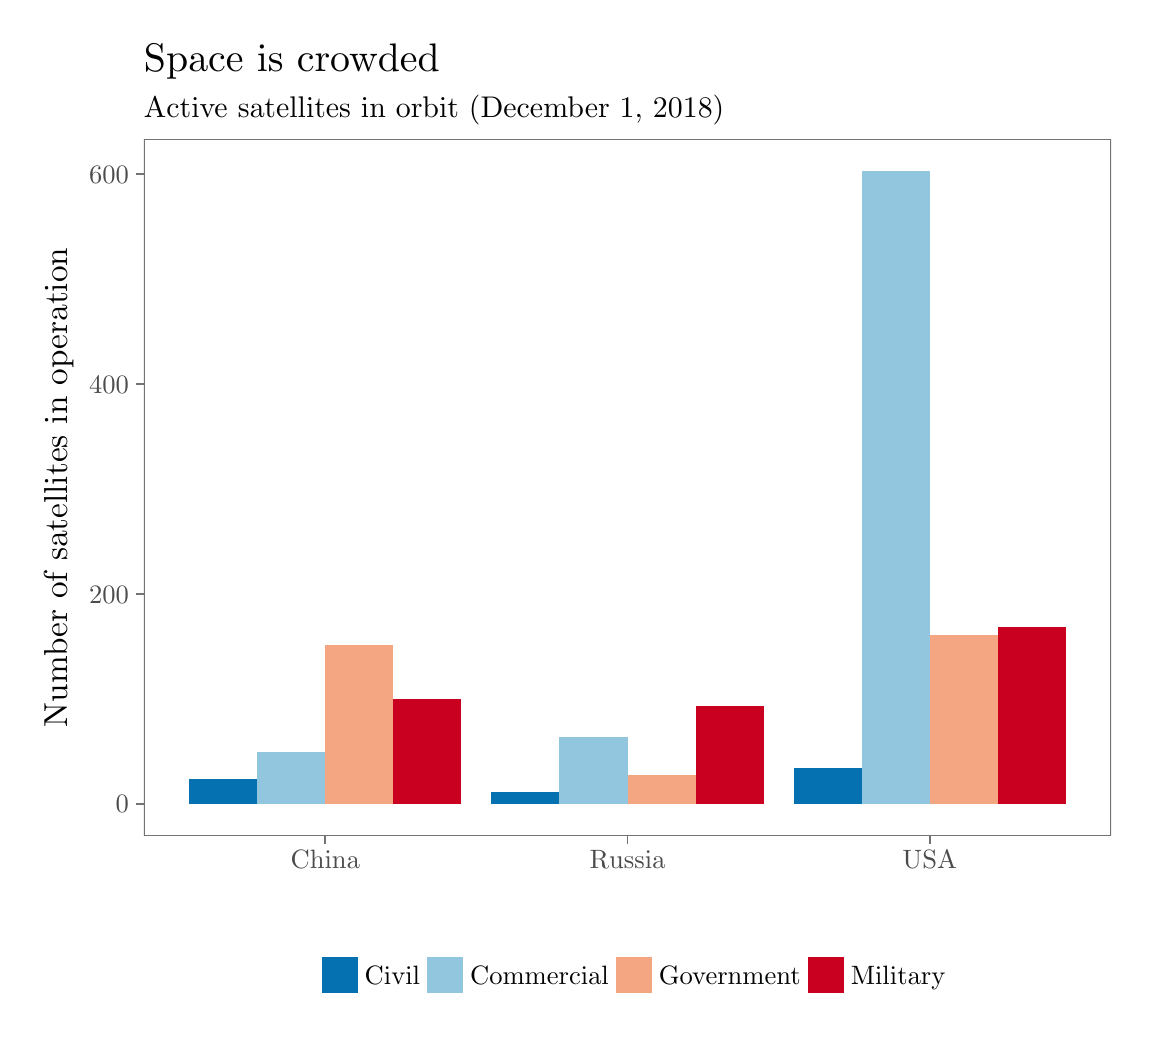
\begin{tikzpicture}[x=1pt,y=1pt]
\definecolor{fillColor}{RGB}{255,255,255}
\path[use as bounding box,fill=fillColor,fill opacity=0.00] (0,0) rectangle (397.48,361.35);
\begin{scope}
\path[clip] (  0.00,  0.00) rectangle (397.48,361.35);
\definecolor{drawColor}{RGB}{255,255,255}
\definecolor{fillColor}{RGB}{255,255,255}

\path[draw=drawColor,line width= 0.6pt,line join=round,line cap=round,fill=fillColor] (  0.00,  0.00) rectangle (397.48,361.35);
\end{scope}
\begin{scope}
\path[clip] ( 42.01, 69.49) rectangle (391.48,320.95);
\definecolor{fillColor}{RGB}{255,255,255}

\path[fill=fillColor] ( 42.01, 69.49) rectangle (391.48,320.95);
\definecolor{fillColor}{RGB}{202,0,32}

\path[fill=fillColor] (132.11, 80.92) rectangle (156.68,118.83);
\definecolor{fillColor}{RGB}{244,165,130}

\path[fill=fillColor] (107.53, 80.92) rectangle (132.11,138.17);
\definecolor{fillColor}{RGB}{146,197,222}

\path[fill=fillColor] ( 82.96, 80.92) rectangle (107.53, 99.50);
\definecolor{fillColor}{RGB}{5,113,176}

\path[fill=fillColor] ( 58.39, 80.92) rectangle ( 82.96, 90.02);
\definecolor{fillColor}{RGB}{202,0,32}

\path[fill=fillColor] (241.32, 80.92) rectangle (265.89,116.18);
\definecolor{fillColor}{RGB}{244,165,130}

\path[fill=fillColor] (216.75, 80.92) rectangle (241.32, 91.16);
\definecolor{fillColor}{RGB}{146,197,222}

\path[fill=fillColor] (192.17, 80.92) rectangle (216.75,105.19);
\definecolor{fillColor}{RGB}{5,113,176}

\path[fill=fillColor] (167.60, 80.92) rectangle (192.17, 85.09);
\definecolor{fillColor}{RGB}{202,0,32}

\path[fill=fillColor] (350.53, 80.92) rectangle (375.10,144.61);
\definecolor{fillColor}{RGB}{244,165,130}

\path[fill=fillColor] (325.96, 80.92) rectangle (350.53,141.96);
\definecolor{fillColor}{RGB}{146,197,222}

\path[fill=fillColor] (301.38, 80.92) rectangle (325.96,309.52);
\definecolor{fillColor}{RGB}{5,113,176}

\path[fill=fillColor] (276.81, 80.92) rectangle (301.38, 93.81);
\definecolor{drawColor}{gray}{0.45}

\path[draw=drawColor,line width= 0.6pt,line join=round,line cap=round] ( 42.01, 69.49) rectangle (391.48,320.95);
\end{scope}
\begin{scope}
\path[clip] (  0.00,  0.00) rectangle (397.48,361.35);
\definecolor{drawColor}{gray}{0.30}

\node[text=drawColor,anchor=base east,inner sep=0pt, outer sep=0pt, scale=  0.96] at ( 36.61, 77.62) {0};

\node[text=drawColor,anchor=base east,inner sep=0pt, outer sep=0pt, scale=  0.96] at ( 36.61,153.44) {200};

\node[text=drawColor,anchor=base east,inner sep=0pt, outer sep=0pt, scale=  0.96] at ( 36.61,229.26) {400};

\node[text=drawColor,anchor=base east,inner sep=0pt, outer sep=0pt, scale=  0.96] at ( 36.61,305.08) {600};
\end{scope}
\begin{scope}
\path[clip] (  0.00,  0.00) rectangle (397.48,361.35);
\definecolor{drawColor}{gray}{0.45}

\path[draw=drawColor,line width= 0.6pt,line join=round] ( 39.01, 80.92) --
	( 42.01, 80.92);

\path[draw=drawColor,line width= 0.6pt,line join=round] ( 39.01,156.74) --
	( 42.01,156.74);

\path[draw=drawColor,line width= 0.6pt,line join=round] ( 39.01,232.56) --
	( 42.01,232.56);

\path[draw=drawColor,line width= 0.6pt,line join=round] ( 39.01,308.38) --
	( 42.01,308.38);
\end{scope}
\begin{scope}
\path[clip] (  0.00,  0.00) rectangle (397.48,361.35);
\definecolor{drawColor}{gray}{0.45}

\path[draw=drawColor,line width= 0.6pt,line join=round] (107.53, 66.49) --
	(107.53, 69.49);

\path[draw=drawColor,line width= 0.6pt,line join=round] (216.75, 66.49) --
	(216.75, 69.49);

\path[draw=drawColor,line width= 0.6pt,line join=round] (325.96, 66.49) --
	(325.96, 69.49);
\end{scope}
\begin{scope}
\path[clip] (  0.00,  0.00) rectangle (397.48,361.35);
\definecolor{drawColor}{gray}{0.30}

\node[text=drawColor,anchor=base,inner sep=0pt, outer sep=0pt, scale=  0.96] at (107.53, 57.48) {China};

\node[text=drawColor,anchor=base,inner sep=0pt, outer sep=0pt, scale=  0.96] at (216.75, 57.48) {Russia};

\node[text=drawColor,anchor=base,inner sep=0pt, outer sep=0pt, scale=  0.96] at (325.96, 57.48) {USA};
\end{scope}
\begin{scope}
\path[clip] (  0.00,  0.00) rectangle (397.48,361.35);
\definecolor{drawColor}{RGB}{1,2,2}

\node[text=drawColor,rotate= 90.00,anchor=base,inner sep=0pt, outer sep=0pt, scale=  1.20] at ( 14.26,195.22) {Number of satellites in operation};
\end{scope}
\begin{scope}
\path[clip] (  0.00,  0.00) rectangle (397.48,361.35);
\definecolor{fillColor}{RGB}{255,255,255}

\path[fill=fillColor] ( 96.23,  6.00) rectangle (337.26, 31.84);
\end{scope}
\begin{scope}
\path[clip] (  0.00,  0.00) rectangle (397.48,361.35);
\definecolor{fillColor}{RGB}{255,255,255}

\path[fill=fillColor] (105.53, 11.69) rectangle (119.99, 26.14);
\end{scope}
\begin{scope}
\path[clip] (  0.00,  0.00) rectangle (397.48,361.35);
\definecolor{fillColor}{RGB}{5,113,176}

\path[fill=fillColor] (106.24, 12.40) rectangle (119.27, 25.43);
\end{scope}
\begin{scope}
\path[clip] (  0.00,  0.00) rectangle (397.48,361.35);
\definecolor{fillColor}{RGB}{255,255,255}

\path[fill=fillColor] (143.59, 11.69) rectangle (158.05, 26.14);
\end{scope}
\begin{scope}
\path[clip] (  0.00,  0.00) rectangle (397.48,361.35);
\definecolor{fillColor}{RGB}{146,197,222}

\path[fill=fillColor] (144.31, 12.40) rectangle (157.34, 25.43);
\end{scope}
\begin{scope}
\path[clip] (  0.00,  0.00) rectangle (397.48,361.35);
\definecolor{fillColor}{RGB}{255,255,255}

\path[fill=fillColor] (211.81, 11.69) rectangle (226.26, 26.14);
\end{scope}
\begin{scope}
\path[clip] (  0.00,  0.00) rectangle (397.48,361.35);
\definecolor{fillColor}{RGB}{244,165,130}

\path[fill=fillColor] (212.52, 12.40) rectangle (225.55, 25.43);
\end{scope}
\begin{scope}
\path[clip] (  0.00,  0.00) rectangle (397.48,361.35);
\definecolor{fillColor}{RGB}{255,255,255}

\path[fill=fillColor] (281.16, 11.69) rectangle (295.61, 26.14);
\end{scope}
\begin{scope}
\path[clip] (  0.00,  0.00) rectangle (397.48,361.35);
\definecolor{fillColor}{RGB}{202,0,32}

\path[fill=fillColor] (281.87, 12.40) rectangle (294.90, 25.43);
\end{scope}
\begin{scope}
\path[clip] (  0.00,  0.00) rectangle (397.48,361.35);
\definecolor{drawColor}{RGB}{1,2,2}

\node[text=drawColor,anchor=base west,inner sep=0pt, outer sep=0pt, scale=  0.96] at (121.79, 15.61) {Civil};
\end{scope}
\begin{scope}
\path[clip] (  0.00,  0.00) rectangle (397.48,361.35);
\definecolor{drawColor}{RGB}{1,2,2}

\node[text=drawColor,anchor=base west,inner sep=0pt, outer sep=0pt, scale=  0.96] at (159.86, 15.61) {Commercial};
\end{scope}
\begin{scope}
\path[clip] (  0.00,  0.00) rectangle (397.48,361.35);
\definecolor{drawColor}{RGB}{1,2,2}

\node[text=drawColor,anchor=base west,inner sep=0pt, outer sep=0pt, scale=  0.96] at (228.07, 15.61) {Government};
\end{scope}
\begin{scope}
\path[clip] (  0.00,  0.00) rectangle (397.48,361.35);
\definecolor{drawColor}{RGB}{1,2,2}

\node[text=drawColor,anchor=base west,inner sep=0pt, outer sep=0pt, scale=  0.96] at (297.42, 15.61) {Military};
\end{scope}
\begin{scope}
\path[clip] (  0.00,  0.00) rectangle (397.48,361.35);
\definecolor{drawColor}{RGB}{1,2,2}

\node[text=drawColor,anchor=base west,inner sep=0pt, outer sep=0pt, scale=  1.08] at ( 42.01,328.85) {Active satellites in orbit (December 1, 2018)};
\end{scope}
\begin{scope}
\path[clip] (  0.00,  0.00) rectangle (397.48,361.35);
\definecolor{drawColor}{RGB}{1,2,2}

\node[text=drawColor,anchor=base west,inner sep=0pt, outer sep=0pt, scale=  1.44] at ( 42.01,345.43) {Space is crowded};
\end{scope}
\end{tikzpicture}

  \label{country_sats}
  \caption{Active satellites, grouped by operating country and purpose}
\end{figure}

\newpage
\printbibliography[heading=subbibliography]

\end{document}
